\documentclass[border=0pt]{standalone}
\usepackage[T1]{fontenc}
\usepackage{lmodern}
\usepackage{pgfplots}
\usepgfplotslibrary{groupplots}
\pgfplotsset{compat=1.18}
\definecolor{f02sg}{HTML}{0072B2}
\definecolor{f02arpls}{HTML}{D55E00}
\begin{document}
\begin{minipage}{181.86mm}
\centering
{\bfseries\fontsize{10}{12}\selectfont P08-F02 Extra Trees / M01 individual-spectrum predictions / Sensitivity (S)}\par\vspace{6mm}
% semantic SHA-256: 4c3507299219d2ce29fd9a2a58f030be1b778fd9bbceb756756ca16d12f674f7
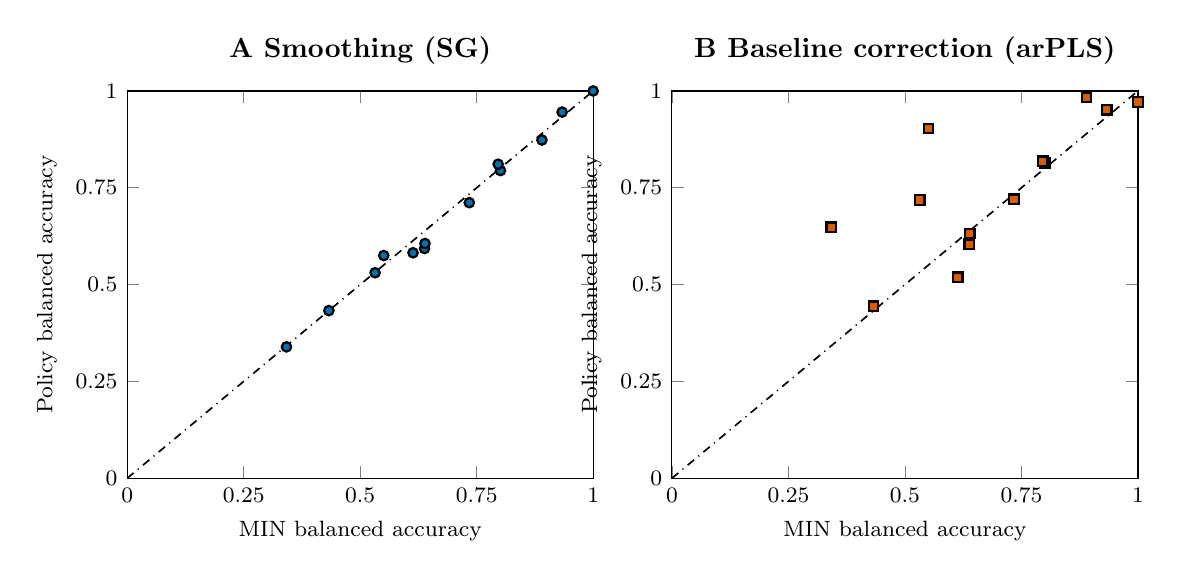
\begin{tikzpicture}
\begin{groupplot}[
  group style={group size=2 by 1, horizontal sep=10mm, vertical sep=6mm},
  width=75mm, height=65mm,
  xmin=0, xmax=1, ymin=0, ymax=1,
  xtick={0,0.25,0.5,0.75,1}, ytick={0,0.25,0.5,0.75,1},
  tick label style={font=\fontsize{8}{9}\selectfont},
  label style={font=\fontsize{8}{9}\selectfont},
  title style={font=\bfseries\fontsize{10}{12}\selectfont},
  xlabel={MIN balanced accuracy}, ylabel={Policy balanced accuracy},
]
\nextgroupplot[title={A  Smoothing (SG)}]
\addplot[black, dash dot, line width=0.6pt, samples=2, domain=0:1, forget plot] {x};
\addplot[only marks, mark=*, mark size=1.7pt, color=f02sg, mark options={draw=black,line width=0.8pt}] coordinates {(0.638095238095238,0.5930952380952381) (0.6133544973544973,0.5822010582010582) (0.6390303030303031,0.6060606060606062) (0.8010606060606061,0.7943939393939395) (0.9333333333333333,0.9454545454545455) (0.3418494623655914,0.33918279569892473) (0.7960317460317461,0.8108465608465609) (1.0,1.0) (0.43280423280423286,0.43280423280423286) (0.5319865319865319,0.5306397306397306) (0.8899999999999999,0.8733333333333333) (0.7341269841269841,0.7115079365079364) (0.5505747126436782,0.575095785440613)};
\nextgroupplot[title={B  Baseline correction (arPLS)}]
\addplot[black, dash dot, line width=0.6pt, samples=2, domain=0:1, forget plot] {x};
\addplot[only marks, mark=square*, mark size=1.7pt, color=f02arpls, mark options={draw=black,line width=0.8pt}] coordinates {(0.638095238095238,0.6041269841269841) (0.6133544973544973,0.518899470899471) (0.6390303030303031,0.6320000000000001) (0.8010606060606061,0.8143939393939394) (0.9333333333333333,0.9515151515151515) (0.3418494623655914,0.6483118279569893) (0.7960317460317461,0.8183862433862433) (1.0,0.9714285714285715) (0.43280423280423286,0.4444444444444445) (0.5319865319865319,0.7185185185185186) (0.8899999999999999,0.9833333333333334) (0.7341269841269841,0.7207142857142858) (0.5505747126436782,0.9030651340996169)};
\end{groupplot}
\end{tikzpicture}
\par\vspace{4pt}
{\fontsize{8}{10}\selectfont RQ-S01: preprocessing and chemical identification. Source-only selection/calibration; selected CNN identity fixed across policies. SG = impulse replacement, smoothing, minmax; arPLS = impulse replacement, baseline correction, minmax. MIN = minimal minmax. Primary: equal contexts within domain, then equal domains. Pooled-fold sensitivity reconstructs each four-fold prediction set before scoring. M01 individual-spectrum predictions; M06 combined predictions per physical sample. M06 averages model probabilities within sample/instrument then equally across instruments, never input spectra or hard labels. 598 original spectra / 69 physical samples / 10 instruments; 557 spectra in 13 held station/instrument domains, 260 contexts. Per-domain independent support in the CSV/table. D1..D13 are lexicographic station/instrument domains, not samples. Diagonal y=x; the 520 points across all panels are paired domain measurements, not 520 independent observations. Claim limit: cannot establish causal background removal or new-instrument performance; no error bars, no significance stars.}\par
\end{minipage}
\end{document}